\documentclass[a4paper]{article}

\usepackage[a4paper, margin=1in]{geometry}
\usepackage{amsmath}
\usepackage{amsfonts}
\usepackage{mathtools}
\usepackage{pgf, tikz}
\usepackage{listings}
\usepackage[colorlinks=true]{hyperref}

\title{
Homework Assignment\\
{\small Dated 2019-11-04, due ???}
}
\author{H. Utku Maden (21947507)}

\begin{document}
    
\maketitle

\section{Topic}

Plot a graph of \(x^2\cdot e^x\) by hand, and in MATLAB (or similar software)
and compare the results.

\section{Hand Plot}

To plot a two-dimensional function by hand one must take the following steps:
\begin{enumerate}
    \item Find the domain of the function.
    \item Determine the intersection points of the function with the $x$
          and $y$ axes.
    \item Find asymptotes, if any.
    \item Analyze the slope of the function on the domain.
    \item Analyze the concavity of the function on the domain.
    \item Construct a unified table providing all relavent information in a
          convenient way.
    \item Graph points of intrests and plot the table accordingly.
\end{enumerate}

\subsection{Domain}

The domain of the function can be found simply by inspecting it's components.

\[
\begin{aligned}
    x^2 & : \mathbb{R} \rightarrow \mathbb{R} \\
    e^x & : \mathbb{R} \rightarrow \mathbb{R} \\
    \text{Therefore } \\
    x^2\cdot e^x & : \mathbb{R} \rightarrow \mathbb{R}
\end{aligned}
\]

\subsection{Intersections}

To find where the function intersects the $y$ axis you must simply
find the value of the function at \(x = 0\).

\[
    \begin{aligned}
        x = 0 & \\
        x^2\cdot e^x & = (0)^2 \cdot e^0 \\
        & = 0\cdot 1 \\
        & = 0 \\
    \end{aligned}
\]

Hence \((0,0)\) is an intersection point of the function.

To find the points the function intersects the $x$ axis one must find the values
of $x$ where $y = 0$. Since the product will be zero if any operand is zero,
one can evaulate the operands of the multiplication separately.

\[
    \begin{aligned}
        x^2 & = 0 \\
        x & \in \left\{0\right\}
    \end{aligned}
\]

\[
    e^x = 0 \text{ has no solution.}
\]

Therefore the only point this function intersects any axes is the origin \((0,0)\).

\subsection{Asymptotes}

Since the function is continuous on \(\mathbb{R}\), no vertical asymptotes
exist.

Also since this function only consists of the product of a polynomial 
and a exponential function, no slant asymptote exists.

For horizontal asymptotes we will evaluate 
\(\lim_{x \rightarrow \pm\infty} {x^2\cdot e^x}\).

\[
    \begin{aligned}
        \lim_{x\rightarrow +\infty} {x^2 \cdot e^x} &
        = \lim_{x\rightarrow +\infty} {x^2} \cdot 
          \lim_{x\rightarrow +\infty} {e^x} \\
        & = \lim_{x\rightarrow +\infty} \infty \cdot \infty \\
        & = +\infty
    \end{aligned}
\]

Thus, no horizontal asymptote exists in the positive direction.

\paragraph{The Asymptote}
\[
    \lim_{x\rightarrow -\infty} {x^2 \cdot e^x}
    = \lim_{x\rightarrow -\infty} {\infty\cdot 0}
\]

We must use the L'Hospital Rule to solve this indeterminity.

\[
    \begin{aligned}
        \lim_{x\rightarrow -\infty} {x^2 \cdot e^x} &
        = \lim_{x\rightarrow -\infty} \frac{x^2}{e^{-x}} \\
        & = \lim_{x\rightarrow -\infty} 
                \frac{ {d(x^2)} / {dx}}
                     { {d(e^{-x})} / {dx}} \\
        & = \lim_{x\rightarrow -\infty}
                \frac{ 2x }
                     { -e^{-x} } \\
        & = \lim_{x\rightarrow -\infty}
                \frac{-\infty}{-\infty}
    \end{aligned}
\]

Again this results in a condition we must use L'Hospital Rule to resolve.

\[
    \begin{aligned}
        \lim_{x\rightarrow -\infty} {x^2 \cdot e^x} &
        = \lim_{x\rightarrow -\infty}
                \frac{ 2x }
                     { -e^{-x} } \\
        & = \lim_{x\rightarrow -\infty}
                 \frac{d(2x)/dx}
                      {d(-e^{-x})/dx} \\
        & = \lim_{x\rightarrow -\infty}
                 \frac{2}
                      {e^{-x}} \\
        & = \lim_{x\rightarrow -\infty}
                \frac{2}
                     {\infty} \\
        & = 0
    \end{aligned}
\]

Hence, there is an asymptote in the negative direction at \(y = 0\)

\subsection{Slope}

Finding the slope of the function is another integral part of
plotting a function. First, one must derive the function.

\[
    \begin{aligned}
        \frac{d(x^2\cdot e^x)}{dx} &
          = (2x)(e^x) + (x^2)(e^x) \\
        & = (e^x)(x^2 + 2x) \\
        & = x(e^x)(x+2)
    \end{aligned}
\]

Now we will evaluate the slope with the given derivative.

\[
    \begin{split}
        f'(x) = 0 = x(e^x)(x+2) = 0 \\
        x \in \left\{0, -2\right\}
    \end{split}
\]

So the slope of the function is as so:

\[
    - \infty \xrightarrow{\text{increasing}} -2 \xrightarrow[\text{decreasing}]{} 0 \xrightarrow{\text{increasing}} +\infty
\]

We can also see that $-2$ is a local maximum and $0$ is a local minimum.

\subsection{Convaity}

The concavity of the function is another integral part of plotting a graph.
Just like the slope, this is found by a derivative, in fact the second
derivative of the function.

Since \(f'(x) = (xe^x)(x+2)\) (see above) we can easily find the second derivative.

\[
    \begin{aligned}
        f''(x) & = (xe^x)'\cdot(x+2) + (xe^x) \\
        & = (1\cdot e^x + xe^x)(x+2) + (xe^x) \\
        & = (e^x + xe^x)(x+2) + (xe^x) \\
        & = xe^x + 2e^x + x^2 e^x + 2xe^x + xe^x \\
        & = x^2e^x + 4xe^x + 2e^x \\
        & = e^x(x^2 + 4x + 2)
    \end{aligned}
\]

After finding the functions, we must find the solutions of \(f''(x)\).

\[
    e^x \text{has not solution.}
\]

We must use the quadratic formula to solve \(x^2 + 4x + 2\).

\[
    \begin{split}
        \Delta = 4^2 - 4 \cdot 1 \cdot 2 = 8 \\
        \sqrt{\Delta} = 2\sqrt{2}
    \end{split}
\]

\[
    x_1 = \frac{-4-2\sqrt{2}}{2} \approx -3.41 \; x_2 = \frac{-4+2\sqrt{2}}{2} \approx -0.59
\]

So the concavity of the function is like this:

\[
    -\infty \xrightarrow{\text{upward}} -3.41 \xrightarrow[\text{downward}]{} -0.59 \xrightarrow{\text{upward}} + \infty
\]

We can also see that \(-3.41\) and \(-0.59\) are inflection points.

\subsection{Unified Table}

With the information we have found above, we must build a unified table
so we can plot the function accurately and conveniently.

\begin{center}
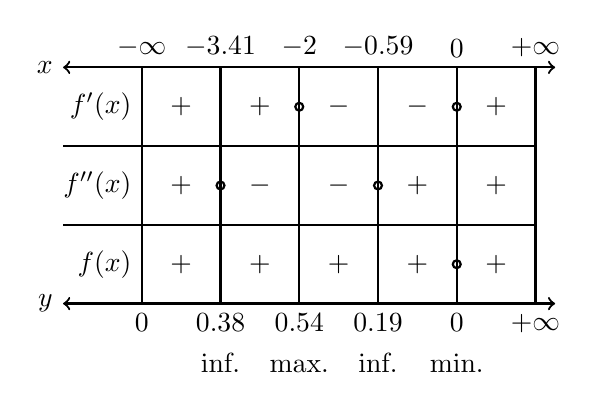
\begin{tikzpicture}
    \draw[thick, <->] 
        (0,0) -- (6.25,0)
        node [left] at (0,0) {$x$}
        node [above] at (1,0) {$-\infty$}
        node [above] at (2,0) {$-3.41$}
        node [above] at (3,0) {$-2$}
        node [above] at (4,0) {$-0.59$}
        node [above] at (5,0) {$0$}
        node [above] at (6,0) {$+\infty$};
    
    \draw[thick, <->]
        (0,-3) -- (6.25, -3)
        node [left] at (0,-3) {$y$}
        node [below] at (1,-3) {$0$}
        node [below] at (2,-3) {$0.38$}
        node [below] at (3,-3) {$0.54$}
        node [below] at (4,-3) {$0.19$}
        node [below] at (5,-3) {$0$}
        node [below] at (6,-3) {$+\infty$}
        ;
    \draw[thick]
        (1,0) -- (1,-3)
        (2,0) -- (2,-3)
        (3,0) -- (3,-3)
        (4,0) -- (4,-3)
        (5,0) -- (5,-3)
        (6,0) -- (6,-3)

        (0,-1) -- (6, -1)
        (0,-2) -- (6, -2)

        node [left] at (1, -0.5) {$f'(x)$}
        node [left] at (1, -1.5) {$f''(x)$}
        node [left] at (1, -2.5) {$f(x)$}
        ;
    
    \draw [thick]
        (3, -0.5) circle [radius=0.5mm]
        (5, -0.5) circle [radius=0.5mm]
        
        node at (1.5, -0.5) {$+$}
        node at (2.5, -0.5) {$+$}
        node at (3.5, -0.5) {$-$}
        node at (4.5, -0.5) {$-$}
        node at (5.5, -0.5) {$+$};
    
    \draw [thick]
        (2, -1.5) circle [radius=0.5mm]
        (4, -1.5) circle [radius=0.5mm]
        
        node at (1.5, -1.5) {$+$}
        node at (2.5, -1.5) {$-$}
        node at (3.5, -1.5) {$-$}
        node at (4.5, -1.5) {$+$}
        node at (5.5, -1.5) {$+$};
    
    \draw [thick]
        (5, -2.5) circle [radius=0.5mm]
        
        node at (1.5, -2.5) {$+$}
        node at (2.5, -2.5) {$+$}
        node at (3.5, -2.5) {$+$}
        node at (4.5, -2.5) {$+$}
        node at (5.5, -2.5) {$+$};
    
        \draw
            node [above] at (2,-4) {inf.}
            node [above] at (3,-4) {max.}
            node [above] at (4,-4) {inf.}
            node [above] at (5,-4) {min.};
    
\end{tikzpicture}
\end{center}

Now we have all the information we need for a plot of the graph.

\section{Computer Plot}

Using a computer to plot the graph of a function is easy. You can use
software such as MATLAB to easily plot graphs, inspect them and create
vector or raster images of them.

I have used GNU Octave because of avaliability, however the scipt is 
MATLAB compatible.

\lstinputlisting[language=Octave]{computer/matplot.m}

\begin{center}
\includegraphics[width=118.8mm]{computer/plot.png}
\end{center}

For the comparison of the plots, the figures are simply 
overlayed in graphics editing software.

\begin{figure}[h!]
    \centering
    \includegraphics[width=118.8mm]{computer/comparison.png}
    \caption{The figures overlayed in software.}
    \label{compare}
\end{figure}

Despite the inaccuracies of the hand plot, Figure \ref{compare} clearly
shows we were able to plot the function successfully.In hand plots,
features of the function are exaggerated unless done in another
approach. Due to this fact, hand plots should not be used in geometric
proofs, but as a reference.

However our hand plot is not missing any feature of the graph. All the 
inflection points, local minimums, local maximums, and intersections are
visible.

{\small
\vspace{10mm}
Visit 
\url{https://github.com/utkumaden/mat_homework/tree/master/2019-11-04} to
analyze the source of this document and the MATLAB script.
}
\end{document}